\subsection{Particle ratios for \tracklet 0--1\%}\label{Sec:ResRat}

QGP-like effects, such as collective flow and strangeness enhancement, affect hadrons of heavier species distinctly. Collective flow will boost heavier particles to larger \pt than lighter particles, and strangeness enhancement in previous measurements was found to scale with the number of strange quarks~\cite{Naturepaper}\cite{alice_newstrangeness}. Due to its low mass, abundant production and lack of strangeness, the pion constitutes a good reference for the QCD physics we are less interested in. Therefore, by studying the \pt-differential particle-to-pion ratios, we can potentially identify QGP-like features in the data.

To be able to observe the quantitative trends with the highest precision, we construct double ratio (DR), as defined in Eq.~\ref{Eq:DR}
\begin{equation}\label{Eq:DR}
\centering
    \left(\frac{{\rm d}N/{\rm d}\pt}{{\rm d}N_\PI/{\rm d}\pt}\right)_{\SOPT} \bigg/ \left(\frac{{\rm d}N/ {\rm d}\pt}{{\rm d}N_\PI/{\rm d}\pt}\right)_{\scaleto{\int}{15pt}\SOPT},
\end{equation}
where the denominator represents the \SOPT-integrated, high-multiplicity event sample. The advantage of the double ratio from an experimental standpoint is that most of the systematic uncertainties will cancel in the ratio between the \SOPT-differential and \SOPT-integrated spectra, for the same species. The double ratios therefore have the best precision in terms of systematic uncertainties of all the data presented in this section, where only the uncorrelated sources listed in Tab.~\ref{tab:systematics_pikp} --~\ref{Tab:SysLong} are applied. For the comparison with MC models, the DR means that focus can be shifted away from the large discrepancies between data and model that exists for most particle species, to test if the quantitative \textit{relative} trends are the same in data and MC. Therefore, we advocate that these comparisons are the ones that are most sensitive to the physics of \SOPT selection.


The \pt-differential relative yield of identified light-flavor hadrons to \PI mesons, as well as the DR, for the \tracklet \topone~multiplicity events are presented for the 10\% \SOPT percentiles in Fig.~\ref{Fig:CombRatioPy} and Fig.~\ref{Fig:CombRatioHer}, compared with PYTHIA 8.2 predictions in the former, and EPOS-LHC and Herwig 7.2 predictions in the latter. 

The DR is presented in the lower panels, showcasing a clear enhancement of strangeness yield in isotropic topologies, and a suppression in jet-like topologies. Remarkably, the DR for all presented particle species decrease significantly for jet-like events. This can be interpreted as most particle ratios being shifted towards higher \pt in jet-like events, i.e. as the \pt of the partonic sub-collisions increase, the same hadrons will be produced with larger \pt. The hadron-to-\PI ratios exhibit a small enhancement of strange-hadron ratios in isotropic events, and a pronounced suppression in jet-like events. This suggests that strange particle production is favored in isotropic topologies. 

In Fig.~\ref{Fig:CombRatioPy}, the default Monash tune of PYTHIA 8.2 quantitatively predicts the interplay between the \SOPT-integrated high-multiplicity events and the \SOPT-differential event classes, but shows large quantitative deviation for most of the measured data. The rope tune does slightly better, in particular for baryons, but the deviation is for both tunes particularly large for the two resonance particles \PHI and \KSTAR. In contrast, neither Herwig 7.2 or EPOS-LHC are able to quantitatively describe the \pt-differential particle-to-\PI ratios, as seen in Fig.~\ref{Fig:CombRatioHer}.

The PYTHIA 8.2 Monash tune and the rope hadronization framework are both able to qualitatively capture the trend between isotropic and jet-like topologies in the DR for all presented light-flavor particles. Remarkably, there is no difference between the PYTHIA 8.2 Monash and the PYTHIA 8.2 Rope curves. Even though the production rates of light-flavor hadrons are different, both variations are able to describe the trends presented for the \SOPT characterized events. EPOS-LHC and Herwig 7.2 are able to qualitatively describe some trends, but are not able to describe the full evolution, mainly towards larger \pt.

By utilizing a narrower event selection, we present the \pt-differential relative yield of identified light-flavor hadrons to \PI mesons, as well as the DR, for the \tracklet \topone ~multiplicity with 1\% \SOPT percentiles in Fig.~\ref{Fig:CombRatioPyEx} and Fig.~\ref{Fig:CombRatioHerEx}. The resonances are excluded from this measurement due to the low number of events in the narrow \SOPT and multiplicity selection. This is an experimental challenge that particularly affects both \PHI and \KSTAR, as the signals are contaminated by large combinatorial backgrounds. Likewise, the large fluctuations in the MC predictions present in Fig.~\ref{Fig:CombRatioPyEx} and Fig.~\ref{Fig:CombRatioHerEx} are driven by an insufficient amount of events in the double-differential selection, compounded by the low production rate of the rare particle yields in the various models.

For all measured particles, the effect of the enhancement and suppression of light-flavor particles relative to pions is stronger when approaching more extreme topologies, in particular the suppression of yield in jet-like events. This is clearly seen both through the single particle-to-\PI ratio, and in the DR, contrasting Fig.~\ref{Fig:CombRatioPy} with Fig.~\ref{Fig:CombRatioPyEx}. In particular, one can note a large suppression of strange hadrons across the entire measured \pt range for events with jet-like topologies. This novel feature suggests that the abundance of strange hadrons in high-multiplicity events are produced in events that are associated to soft physics in terms of the azimuthal topology. This observation also implies that there is a significant amount of high-multiplicity events that reflect the same rates of strangeness production found in low-multiplicity events. ALICE has previously published studies of differential \LA/\kzero production in jets relative to the underlying event (UE), where it was found that the ratio in the jet was far below that of the ratio in the UE~\cite{alice_UE}. This is qualitatively similar to what we observe for the most extreme jet-like events in this study. One could therefore understand the results obtained here as a generalization to jet-dominated events.

The $\rm p/\pi$ peak present for the 99--100\% most isotropic events, as well as in the average 0--1\% high-multiplicity events, is significantly suppressed in 0--1\% jet-like event sample. In conjunction with strangeness suppression, this hints towards a decrease of QGP-like effects in events with extremely jetlike topologies. Furthermore, the discrepancy between the $\rm p/\pi$ and $\rm K/\pi$ ratios at high-\pt is interesting to note, where the isotropic/jet-like ratios meet for the $\rm p/\pi$ while diverging for the $\rm K/\pi$. The underlying mechanism of this effect is currently not fully understood.



\begin{figure}[htbp!]
    \centering
	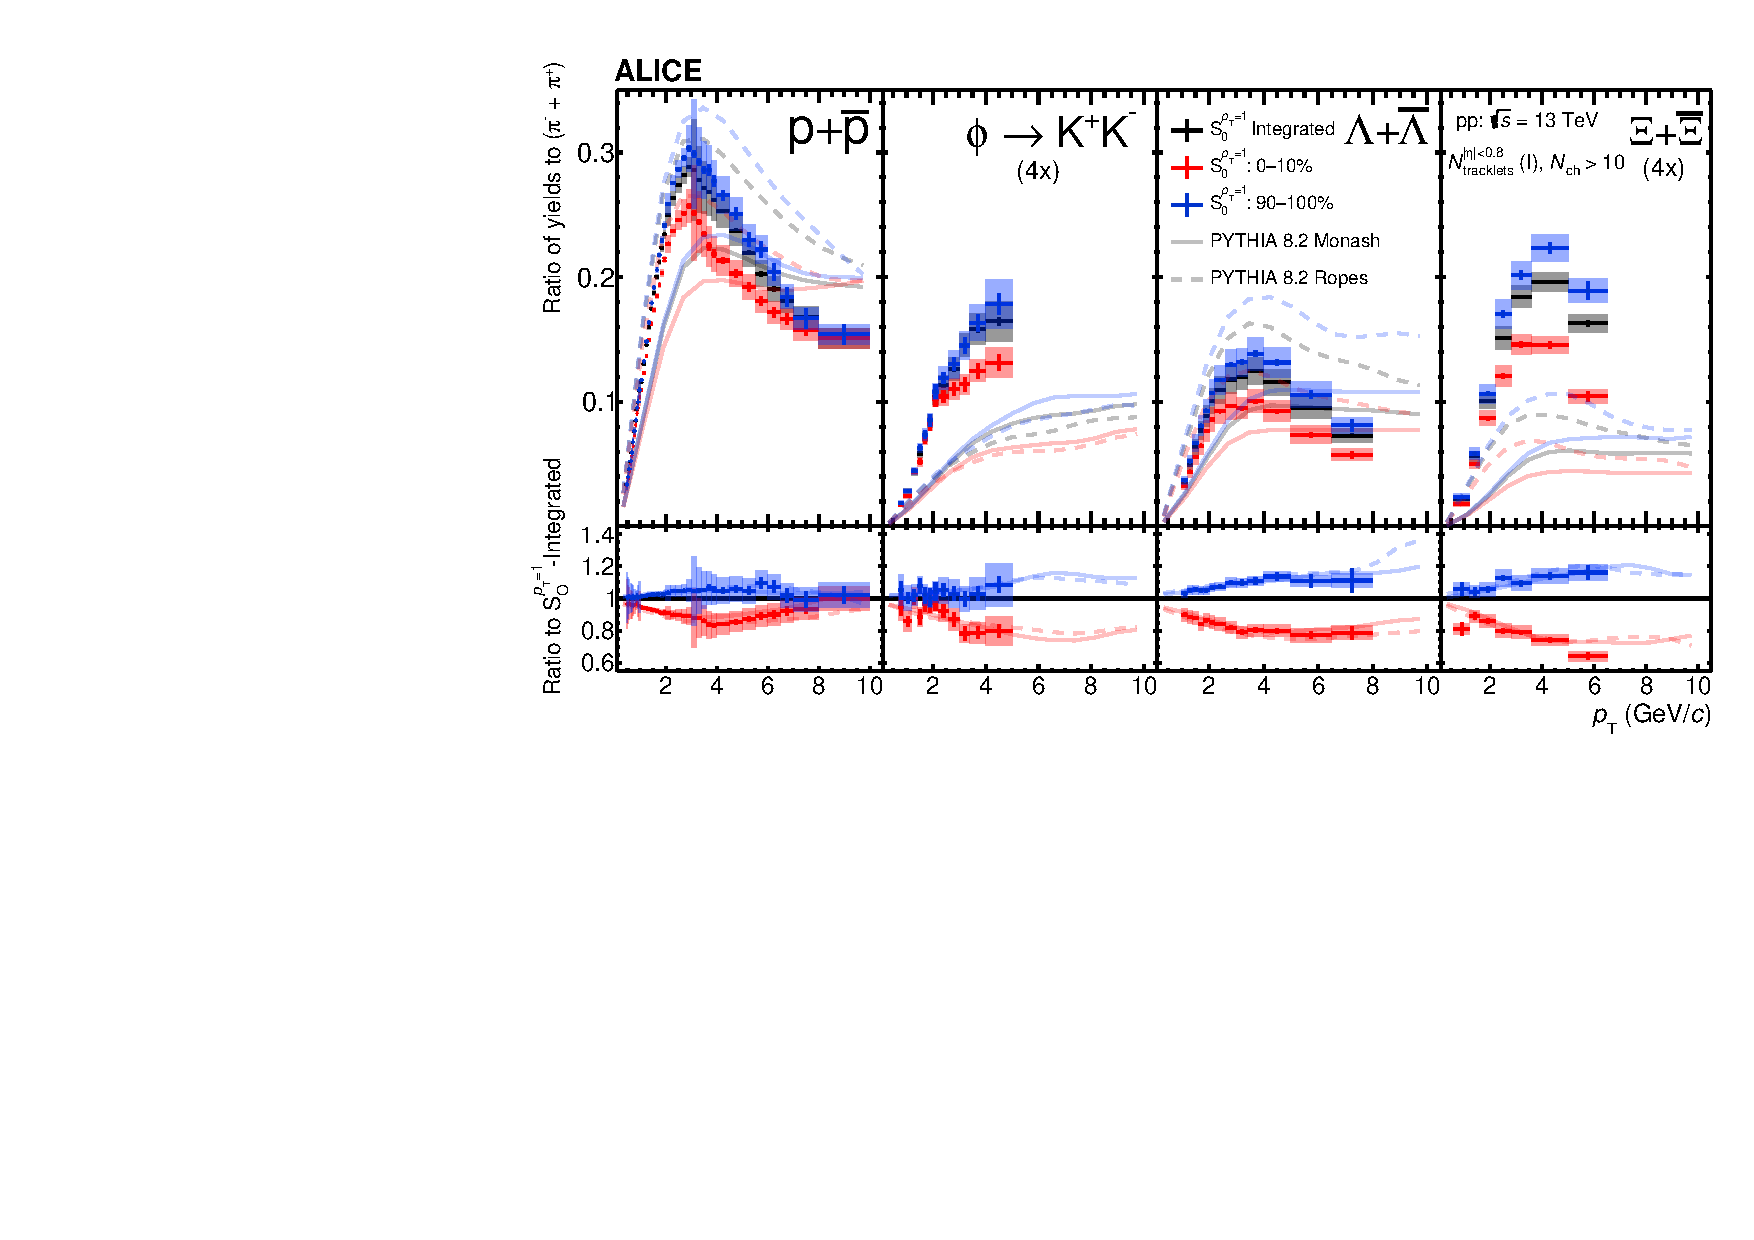
\includegraphics[scale=0.8]{figures/Baryons_SOPT_10_NSPD_1_PY.pdf}
	\newline
     	 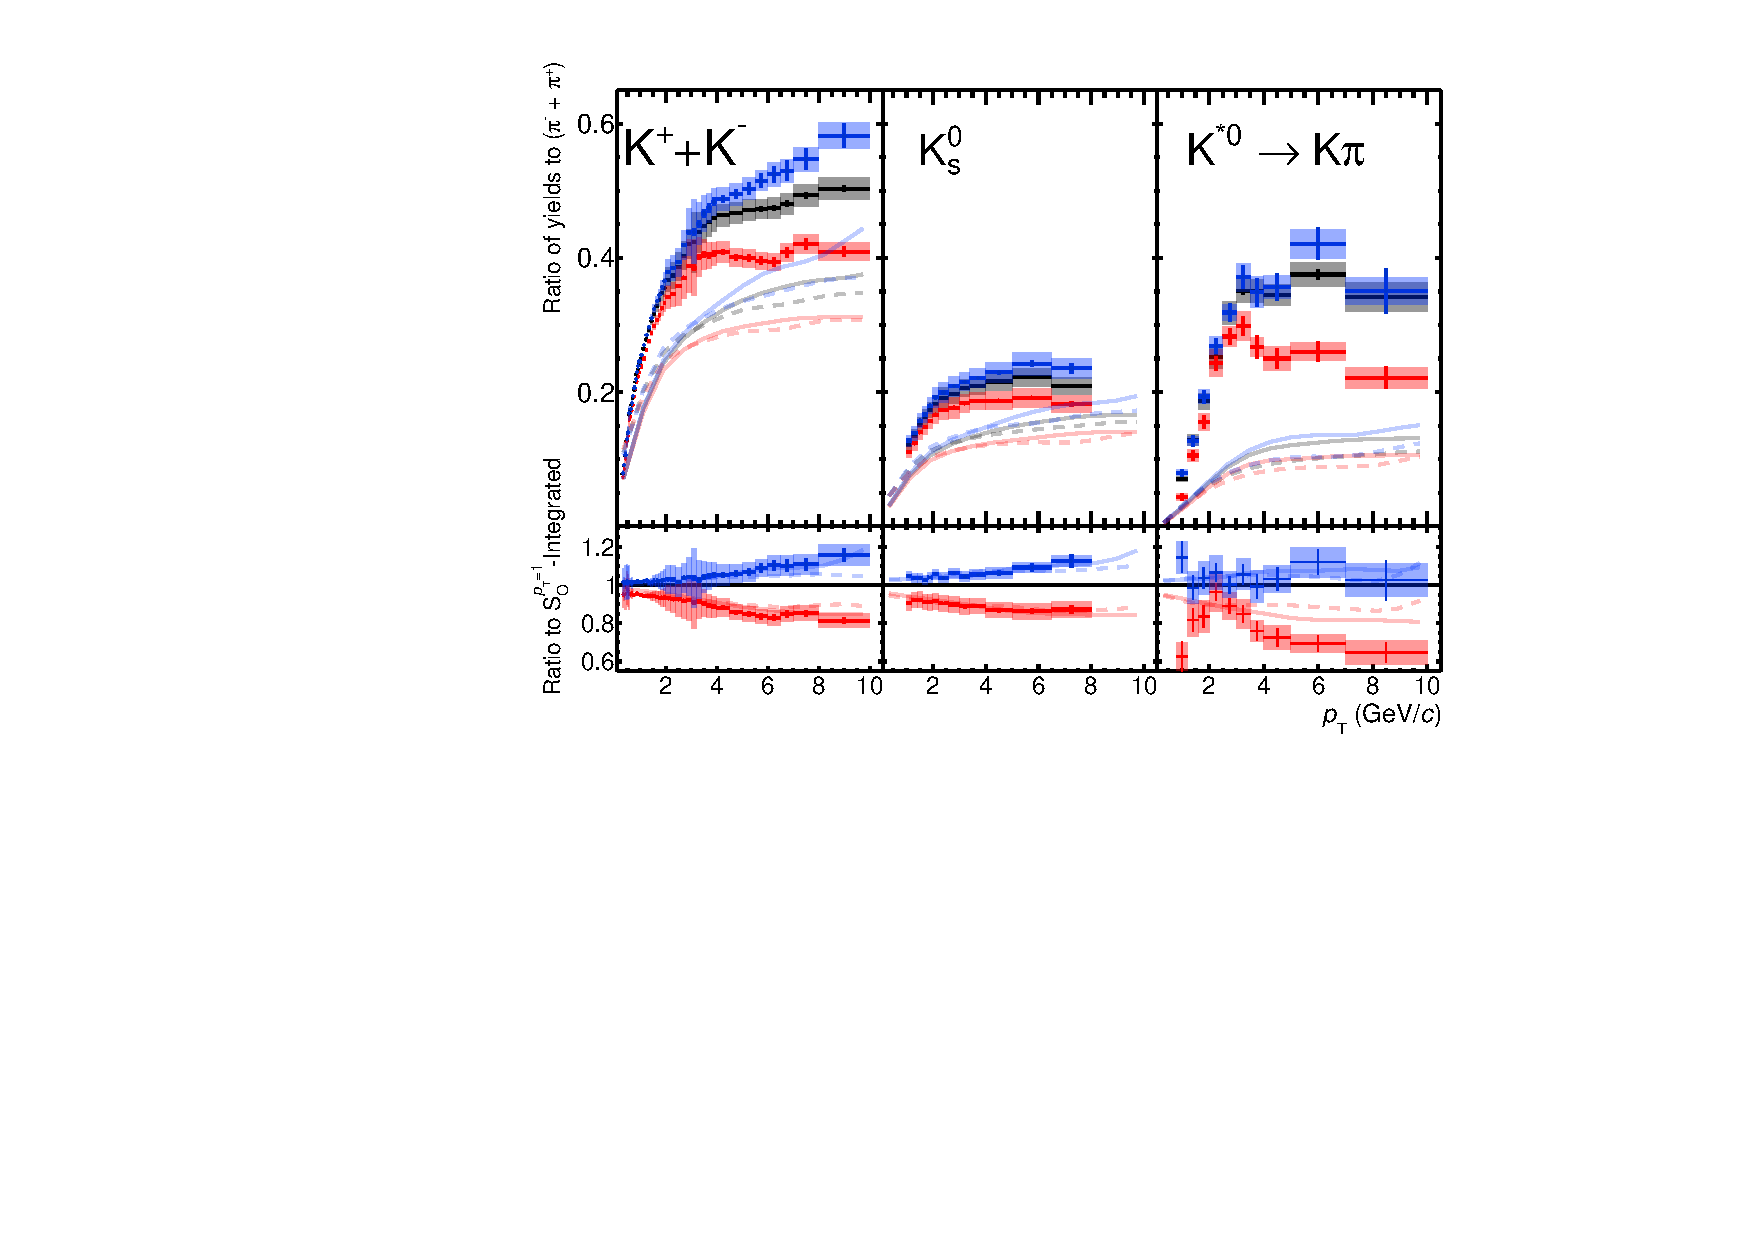
\includegraphics[scale=0.8]{figures/Mesons_SOPT_10_NSPD_1_PY.pdf}
  \caption{Top panels show hadron-to-\PI ratios for 0--10\% \SOPT classes selected for the 0--1\% \tracklet multiplicity events. Bottom panels present the hadron-to-\PI double ratios of \SOPT classes relative to \SOPT integrated high-multiplicity events. Statistical and systematic uncertainties are shown by  bars and boxes, respectively. Experimental results are compared with predictions from PYTHIA 8.2 Monash and Ropes.}   \label{Fig:CombRatioPy}
\end{figure}

\begin{figure}[htbp!]
    \centering
	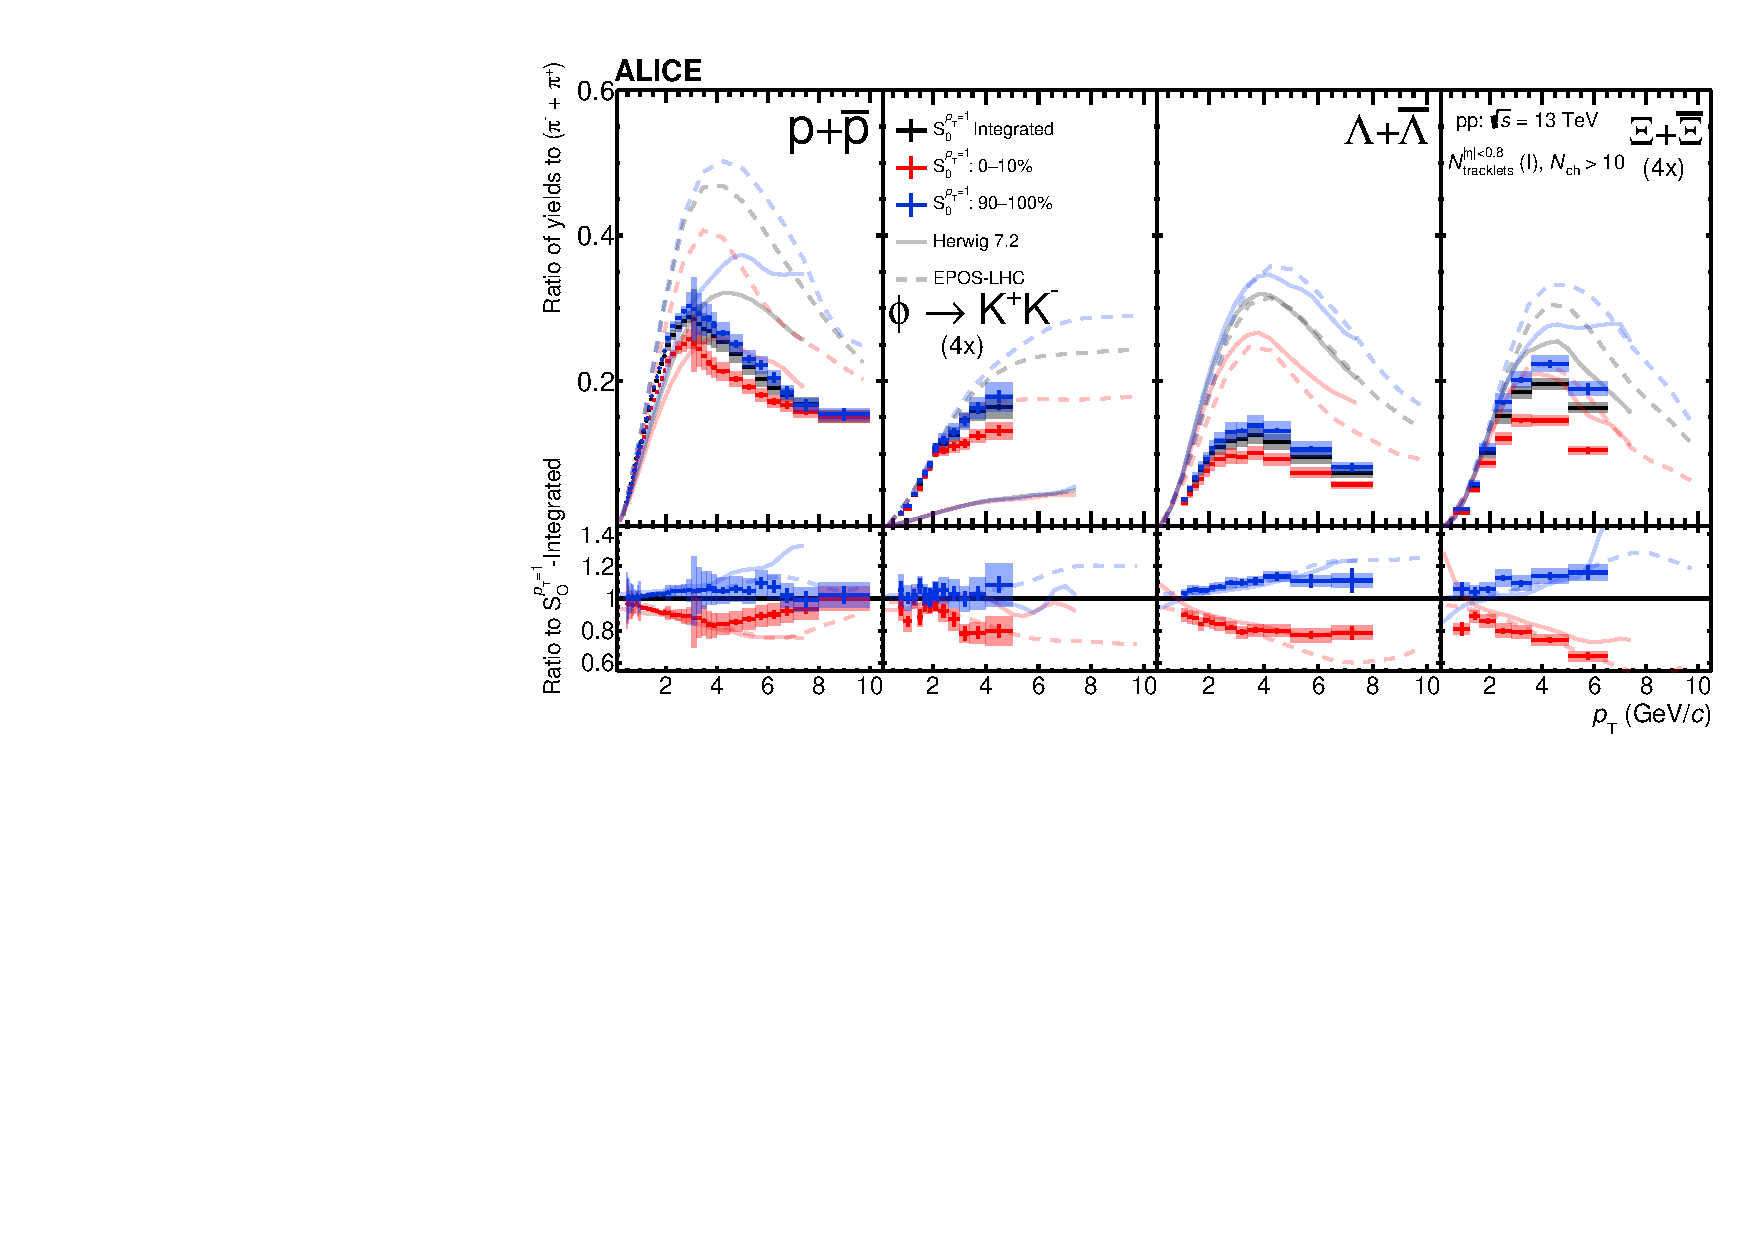
\includegraphics[scale=0.8]{figures/Baryons_SOPT_10_NSPD_1_HW.pdf}
	\newline
	 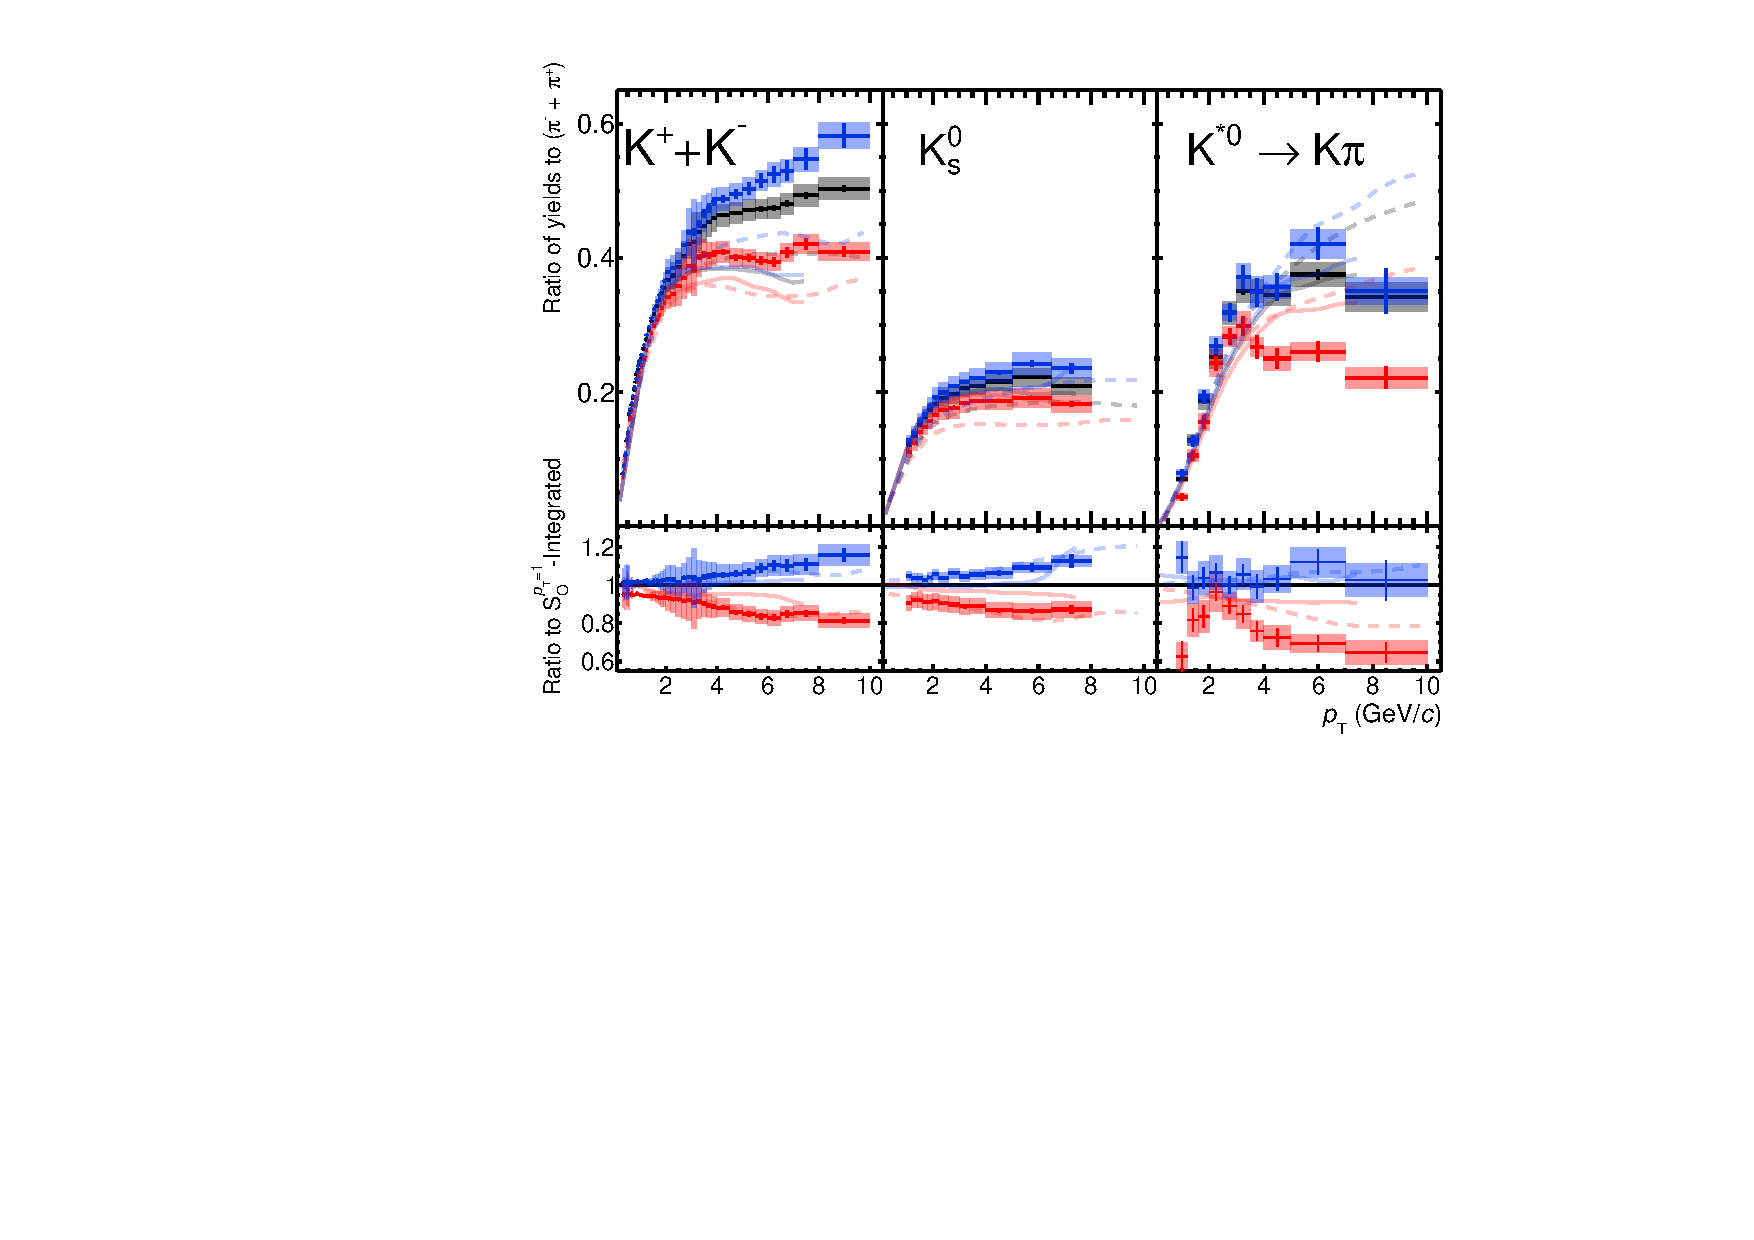
\includegraphics[scale=0.8]{figures/Mesons_SOPT_10_NSPD_1_HW.pdf}
  \caption{Top panels show hadron-to-\PI ratios for 0--10\% \SOPT classes selected for the 0--1\% \tracklet multiplicity events. Figure~\ref{Fig:CombRatioPy} and Fig.~\ref{Fig:CombRatioHer} both contain the same experimental data, but the vertical ranges are modified to accommodate the model predictions. Bottom panels present the hadron-to-\PI double ratios of \SOPT classes relative to \SOPT integrated high-multiplicity events. Statistical and systematic uncertainties are shown by  bars and boxes, respectively. Experimental results are compared with predictions from Herwig 7.2 and EPOS-LHC. The fluctuations present in the Herwig 7.2 predictions are due to statistical limitations.}   \label{Fig:CombRatioHer}
\end{figure}

\begin{figure}[htbp!]
    \centering
	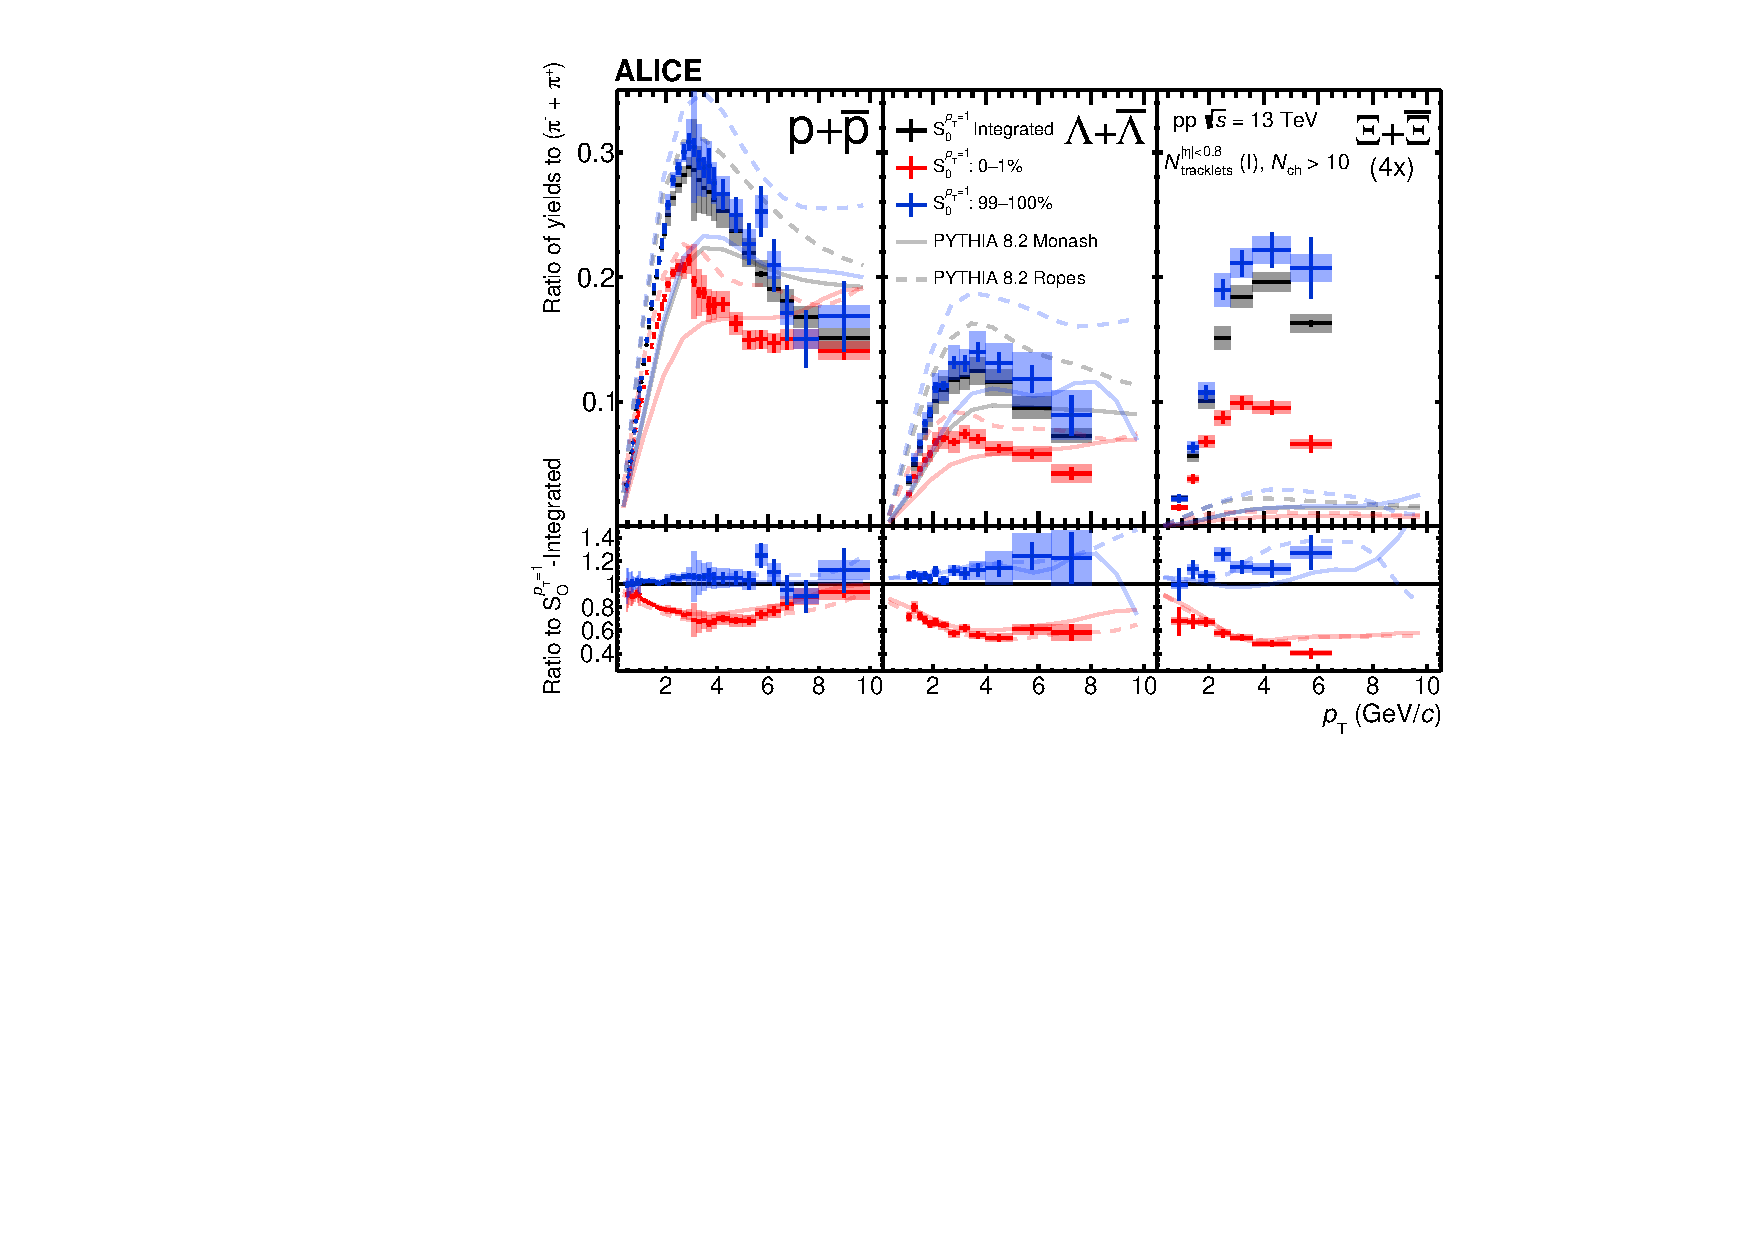
\includegraphics[scale=0.8]{figures/Baryons_SOPT_1_NSPD_1_PY.pdf}
	\newline
	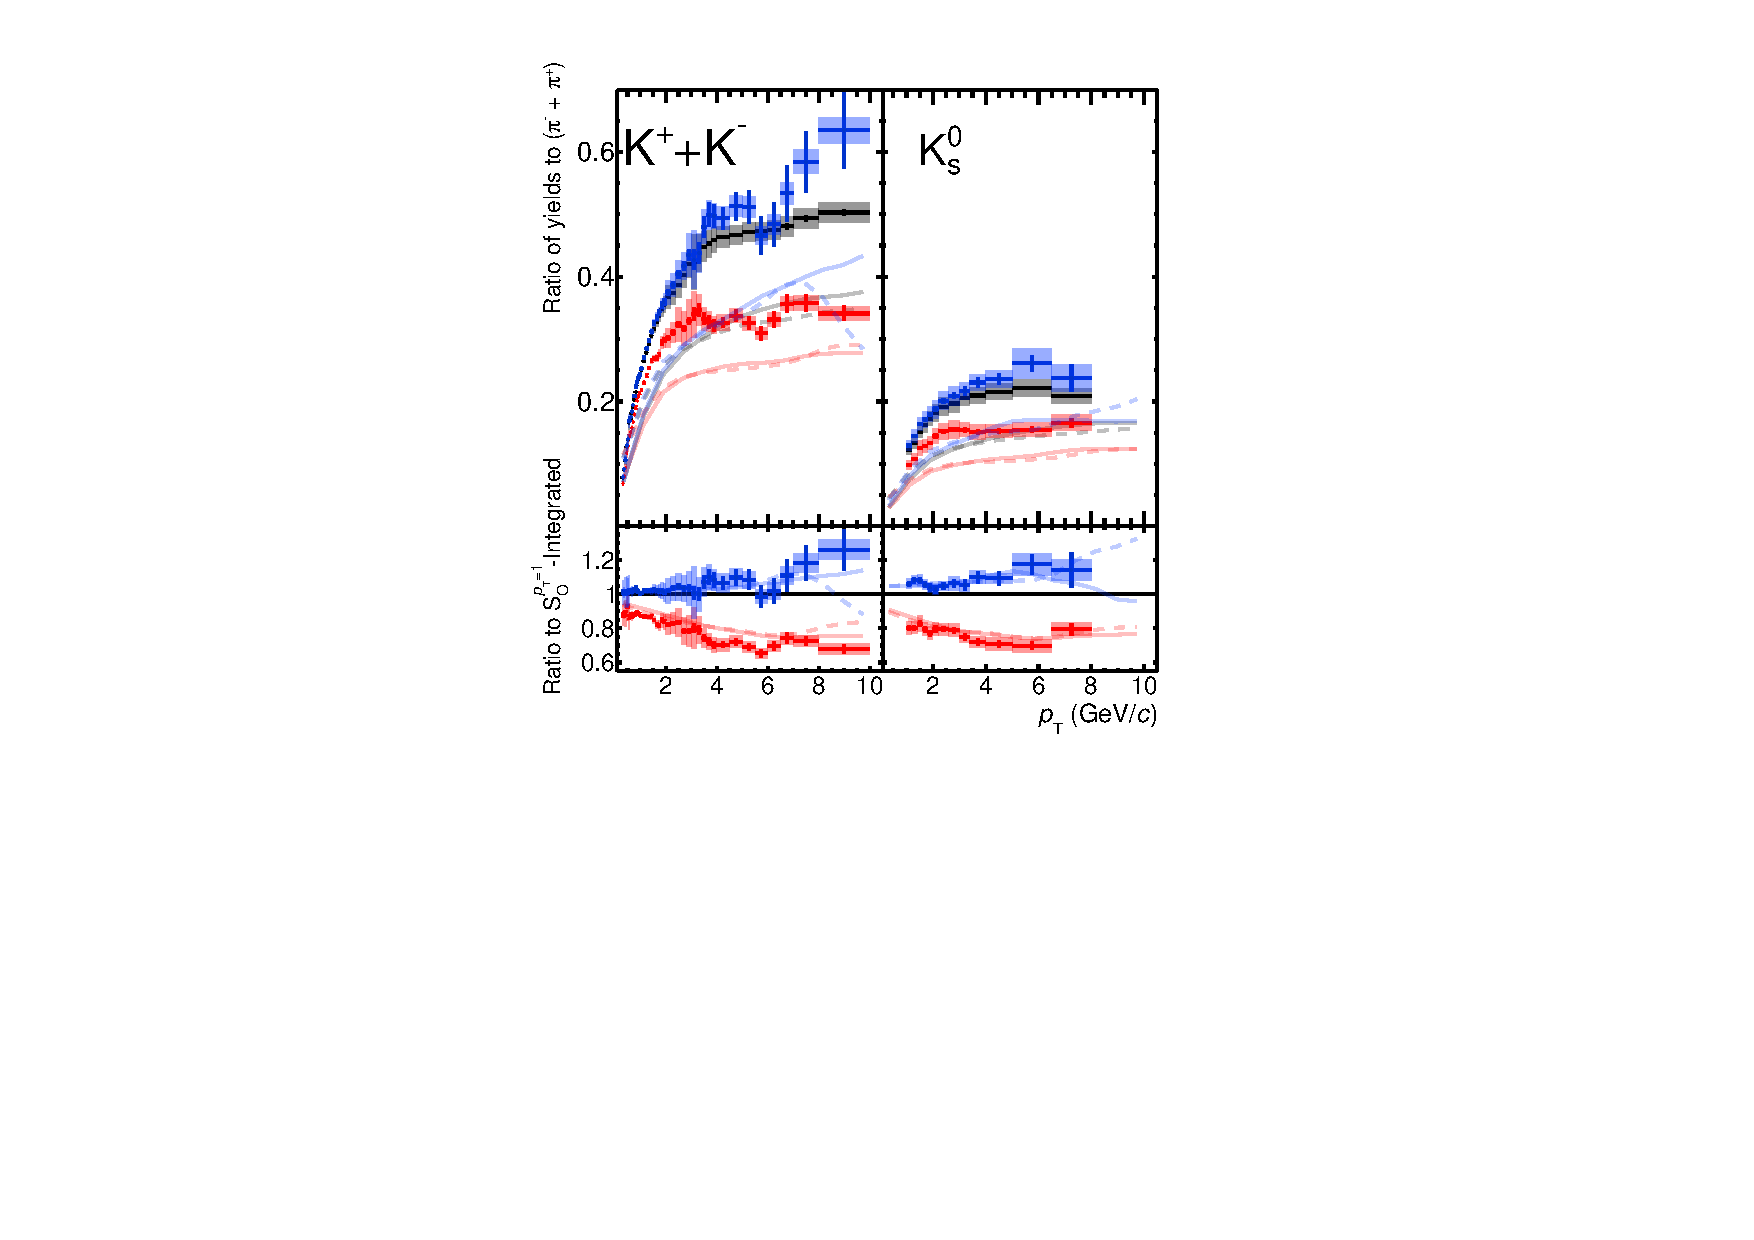
\includegraphics[scale=0.8]{figures/Mesons_SOPT_1_NSPD_1_PY.pdf}
  \caption{Top panels show hadron-to-\PI ratios for 0--1\% \SOPT classes selected for the 0--1\% \tracklet multiplicity events. Bottom panels present the hadron-to-\PI double ratios of \SOPT classes relative to \SOPT integrated high-multiplicity events. Statistical and systematic uncertainties are shown by  bars and boxes, respectively. Experimental results are compared with predictions from PYTHIA 8.2 Monash and Ropes.}
   \label{Fig:CombRatioPyEx}
\end{figure}

\begin{figure}[htbp!]
    \centering
	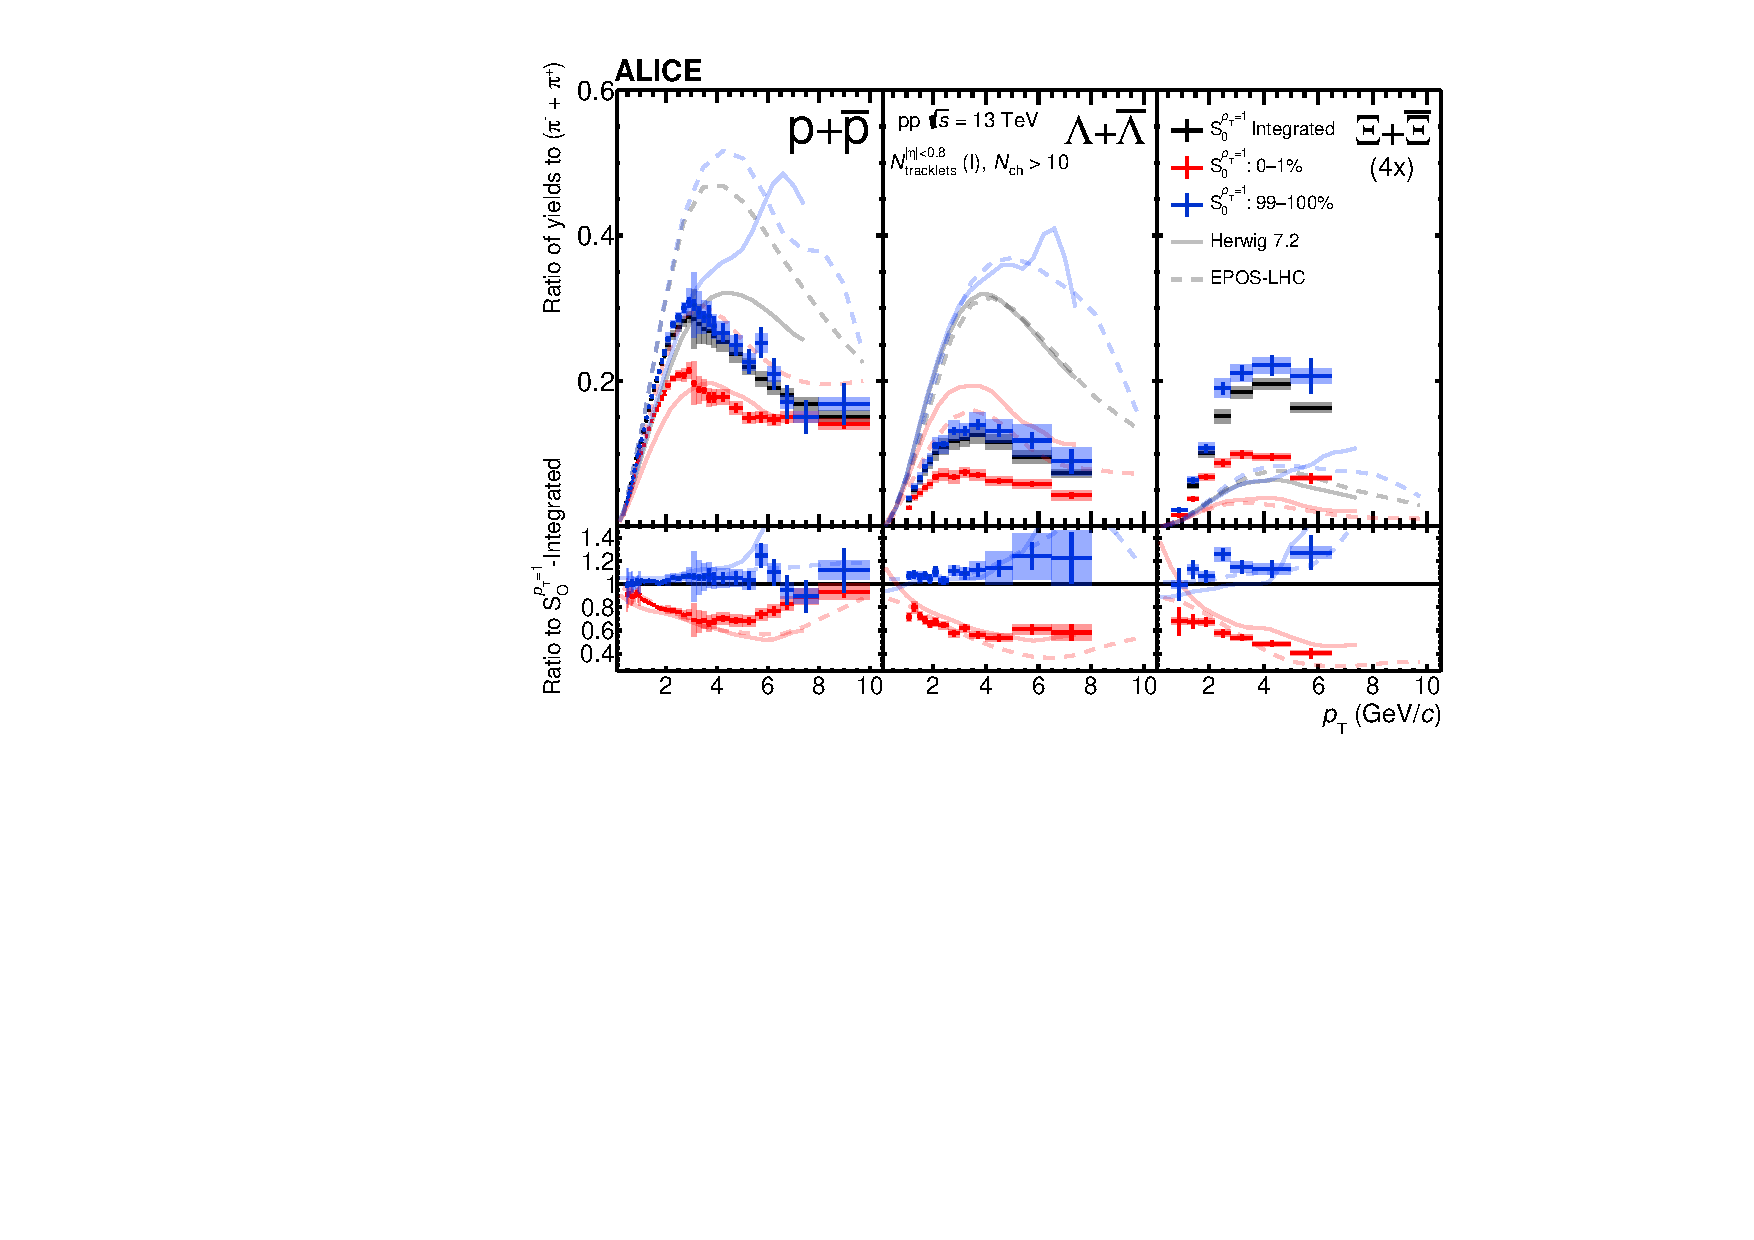
\includegraphics[scale=0.8]{figures/Baryons_SOPT_1_NSPD_1_HW.pdf}
	\newline
	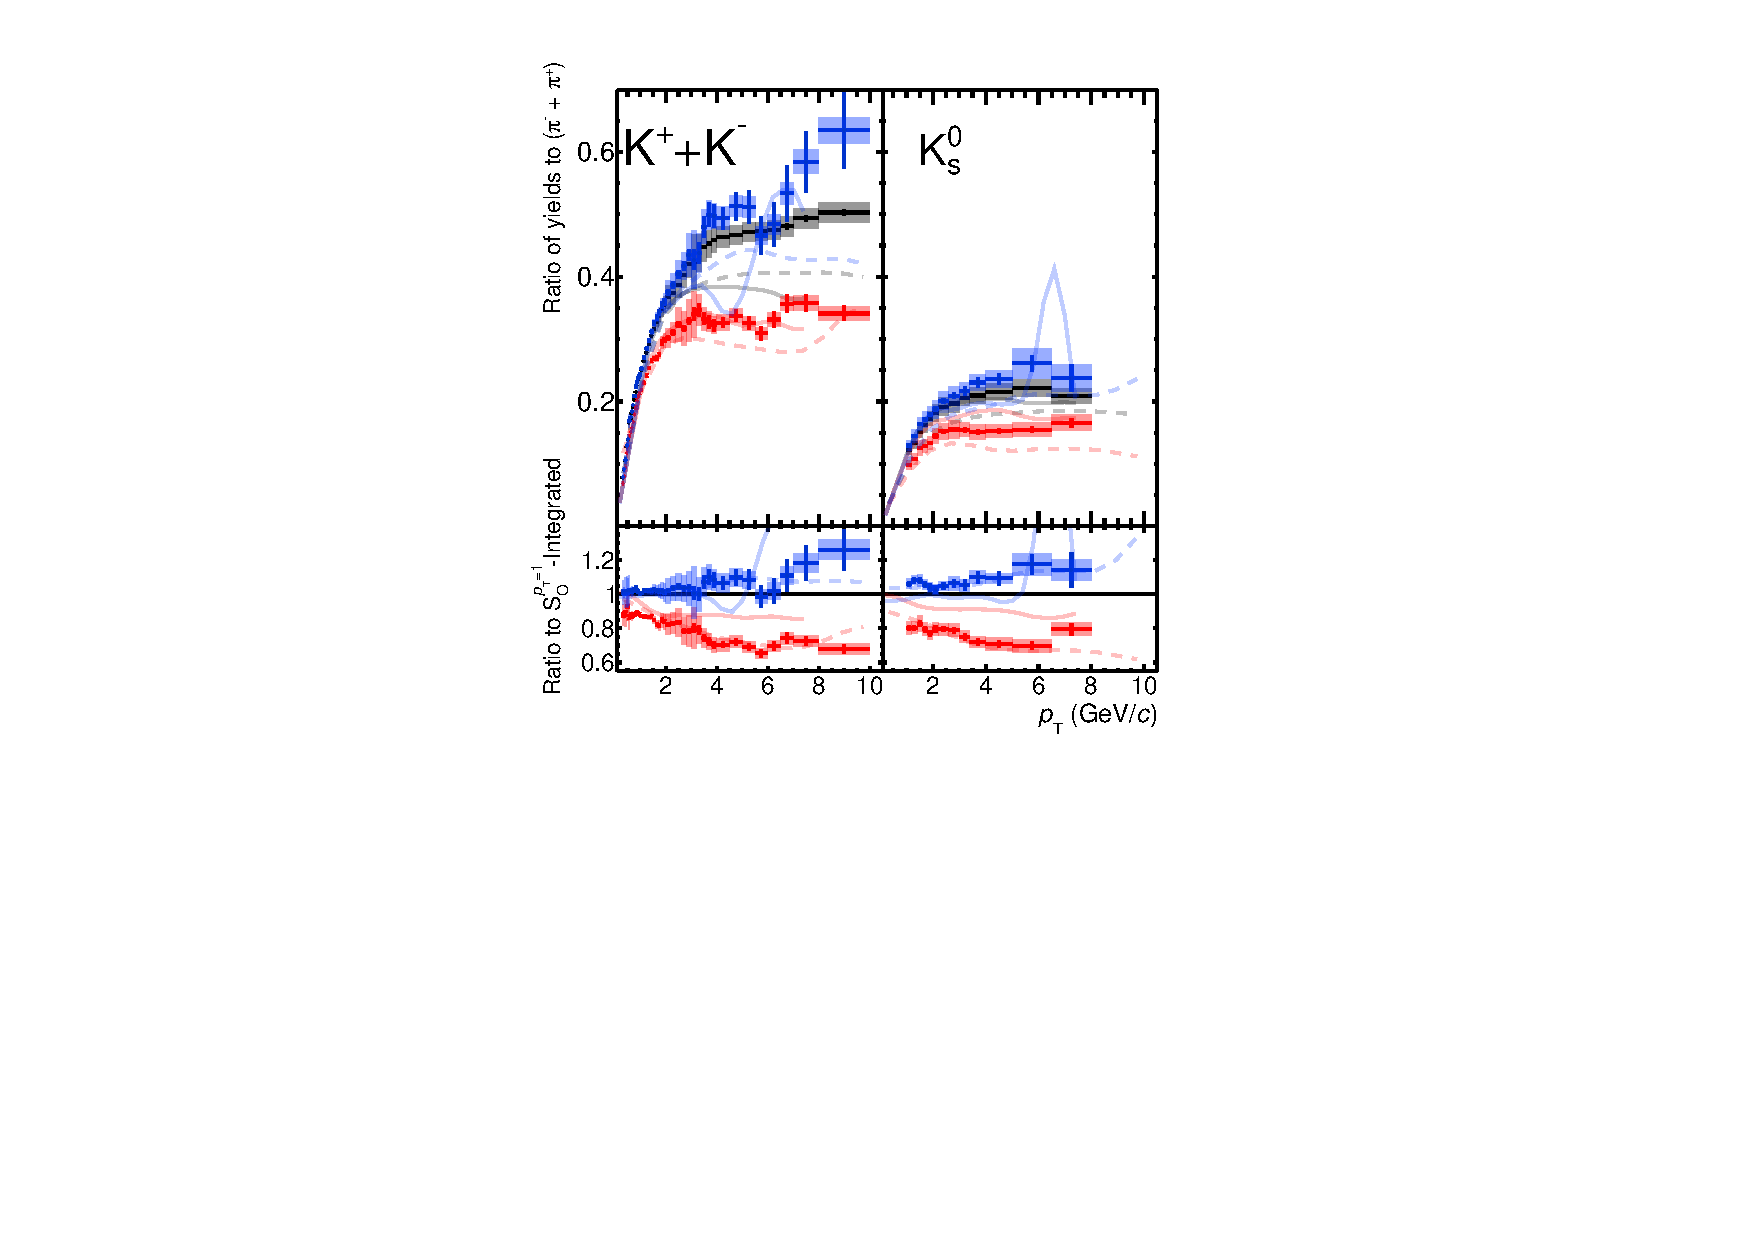
\includegraphics[scale=0.8]{figures/Mesons_SOPT_1_NSPD_1_HW.pdf}
  \caption{Top panels show hadron-to-\PI ratios for 0--1\% \SOPT classes selected for the 0--1\% \tracklet multiplicity events. Figure~\ref{Fig:CombRatioPyEx} and Fig.~\ref{Fig:CombRatioHerEx} both contain the same experimental data, but the vertical ranges are modified to accommodate the model predictions. Bottom panels present the hadron-to-\PI double ratios of \SOPT classes relative to \SOPT integrated high-multiplicity events. Statistical and systematic uncertainties are shown by  bars and boxes, respectively. Experimental results are compared with predictions from Herwig 7.2 and EPOS-LHC. The large fluctuations present in the Herwig 7.2 predictions are due to statistical limitations.}
   \label{Fig:CombRatioHerEx}
\end{figure}

In Fig.~\ref{Fig:CombRatioPyEx}, the two PYTHIA 8.2 predictions are qualitatively able to describe some of the particle-to-\PI ratios for the 1\% \SOPT percentiles, but remarkably underestimate the \pt-differential production of \XI baryons, as well as the isotropic production of both charged and neutral kaons. However, PYTHIA 8.2 is still able to qualitatively describe the interplay between high-multiplicity events, isotropic and jet-like topologies in the DR. Similar to what was observed in Fig.~\ref{Fig:CombRatioHer} for the broader \SOPT selection, EPOS-LHC and Herwig 7.2 are unable to accurately capture the interplay of the DR towards larger \pt. EPOS-LHC and Herwig 7.2 are both able to qualitatively describe most of the observed trends for the charged and neutral kaons in Fig.~\ref{Fig:CombRatioHerEx}, with a slight underestimation of the absolute production rates. However, both model predictions are unable to describe the observed trends for the presented baryons. 

In Fig.~\ref{Fig:Flow}, baryon-to-meson ratios are presented for p/\PI, \LA/\kzero and \XI/\PHI. These ratios are known to be interesting observables, able to highlight features of radial flow and possible recombination~\cite{ALICE:2019hno}. While the \XI/\PHI ratio is not usually associated to measurements of radial flow, phenomenological models have different views of the effective net-strangeness of the \PHI meson. In Lund-string-like models, such as PYTHIA 8.2, the \PHI meson is produced from the fragmentation of $\textrm{s}\bar{\textrm{s}}$ pairs, making it effectively double strange. On the other hand, statistical thermal models typically treats the \PHI meson as having no strangeness, where the production instead is driven by the hadron mass.

The overall trends among the three ratios are qualitatively similar, even as the strangeness content increases from p ($|S|=0$) to \XI ($|S|=2$). Furthermore, one can apply a traditional hypothesis of radial flow in larger collision systems, i.e., that a radial expansion of the system boosts heavier baryons out to high \pt, resulting in a depletion of baryons at low-\pt. In this context, Fig.~\ref{Fig:Flow} highlights an abundance (suppression) of isotropic (jet-like) protons at intermediate \pt in the $p/\PI$ ratio, without the depletion (enhancement) of isotropic (jet-like) protons at low \pt. The origin for the difference in the low-\pt behavior is still unclear, but we suspect that there is an interplay between soft radial flow and the hard suppression in the ratios to pions, observed in the jet-like events through Figs.~\ref{Fig:CombRatioPy}--~\ref{Fig:CombRatioHerEx}. One should keep in mind that the relative systematic uncertainties are smaller than the total systematic uncertainties reported in Fig.~\ref{Fig:Flow}, c.f., Sec.~\ref{Sec:Sys} for further discussion.


Similar trends are observed in the \LA/\kzero ratio, although systematic uncertainties in the lower panel does not allow for a clear conclusion on the interplay between jet-like and isotropic events. The \XI/\PHI ratio suggests that there is a constant enhancement of \XI baryons relative to produced \PHI mesons, within systematic uncertainties.  
\begin{figure}[thbp!]
    \centering
    \hspace{-1.2cm}
    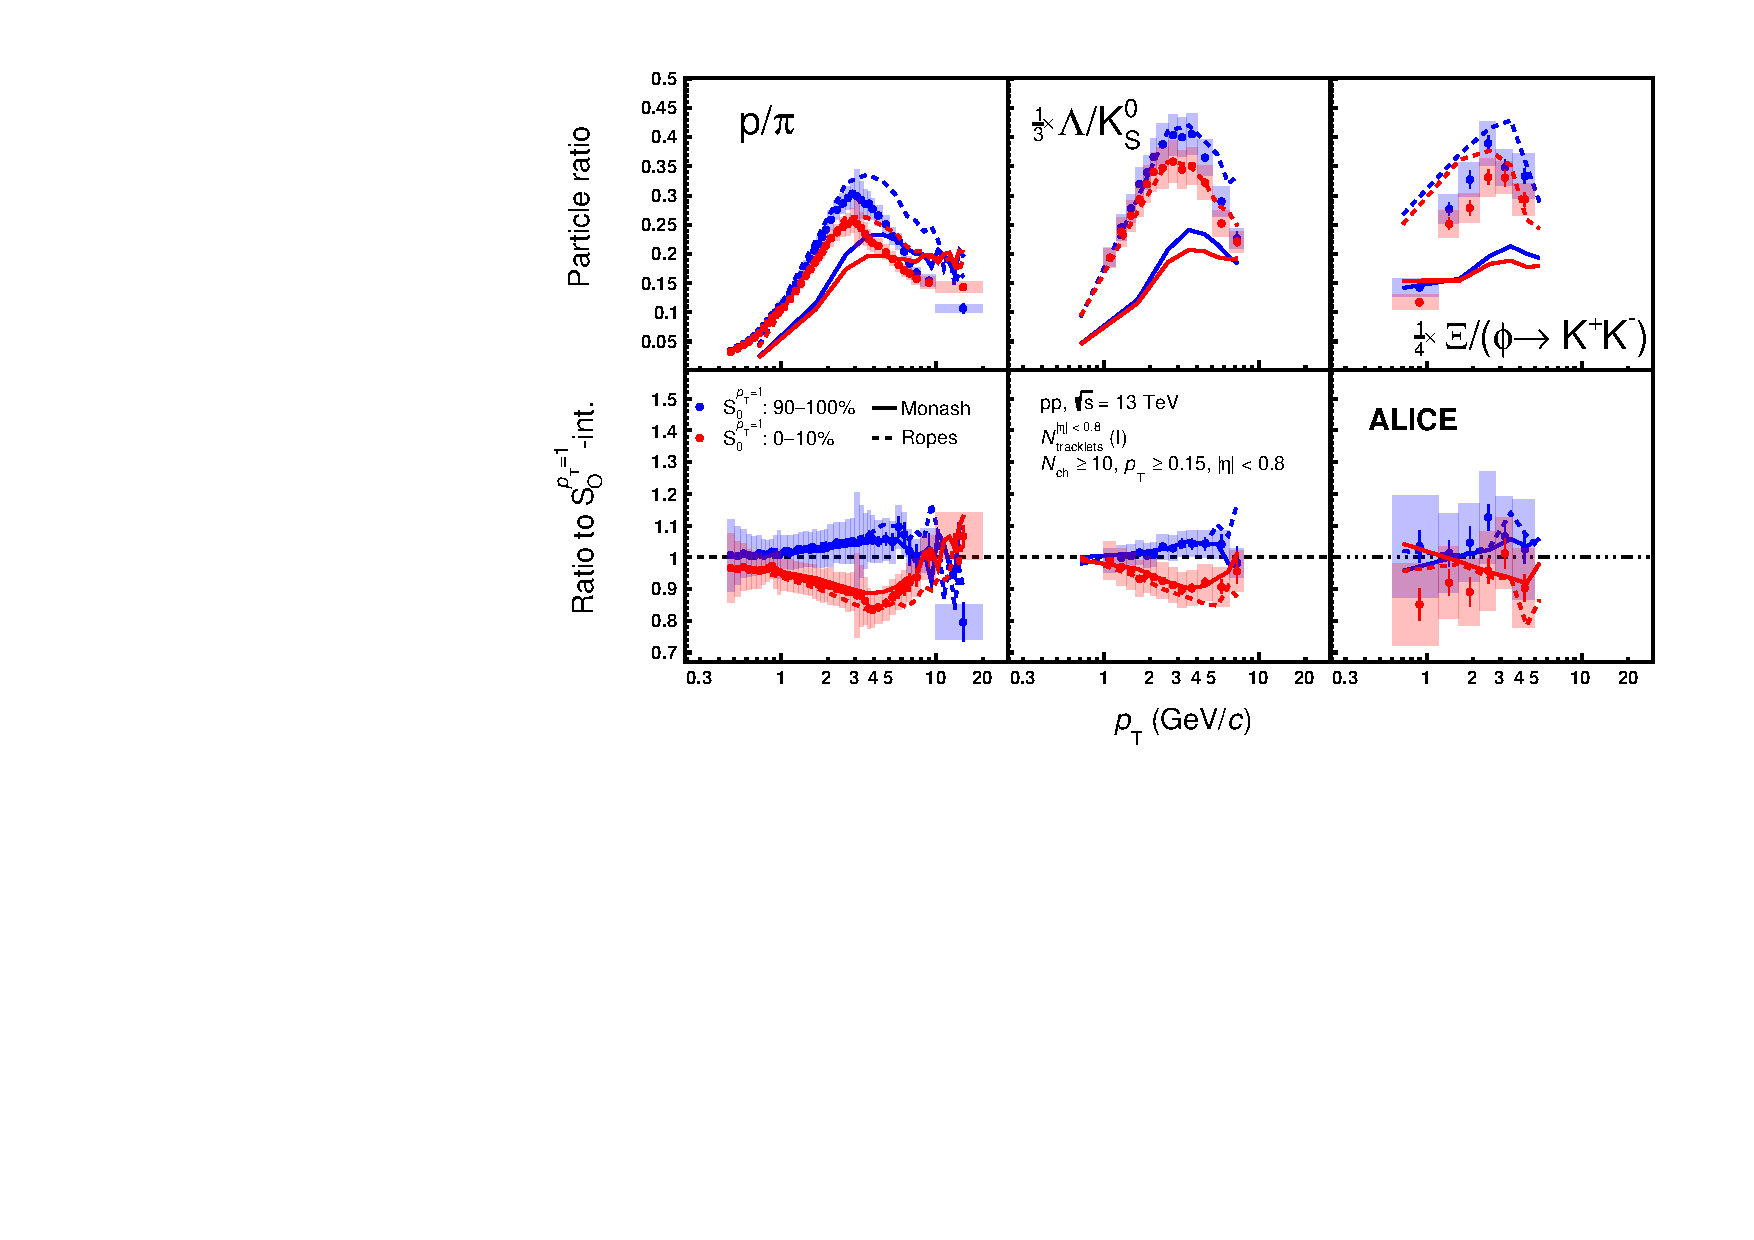
\includegraphics[scale=0.85]{figures/ratiosBaryonMeson.pdf}
    \caption{p/\PI,  \LA/$K$ and \XI/\PHI ratios for different \SOPT classes  are obtained for $0-1\%$ events measured by \tracklet.
    Lower panels show the ratio to \SOPT-integrated event selection.
    Statistical and total systematic uncertainties are shown by bars and boxes, respectively. The curves represent different model predictions of the same measurement. Note that for the p/\PI, the same data points are presented in~\ref{Fig:CombRatioPy}, with an extended \pt range now covering 10--20 \gev. }
    \label{Fig:Flow}
\end{figure}
The rope hadronization framework in PYTHIA 8.2 predicts both the single and double ratios reasonably well. It is remarkable that even though PYTHIA 8.2 Monash fails to predict the single ratios, both PYTHIA 8.2 Monash and Rope predictions show no significant deviations for the double ratios.
The \kzero/K ratios for the different multiplicity estimators are presented in Fig.~\ref{Fig:KtoK}. The ratios highlight a consistency with unity, and showcase no significant \SOPT dependence. These results verify that the modified \SOPT estimator is robust through a data-driven approach, complementing the studies discussed in Sec.~\ref{Sec:SOPT}. 

\begin{figure}[htbp!]
    \centering
    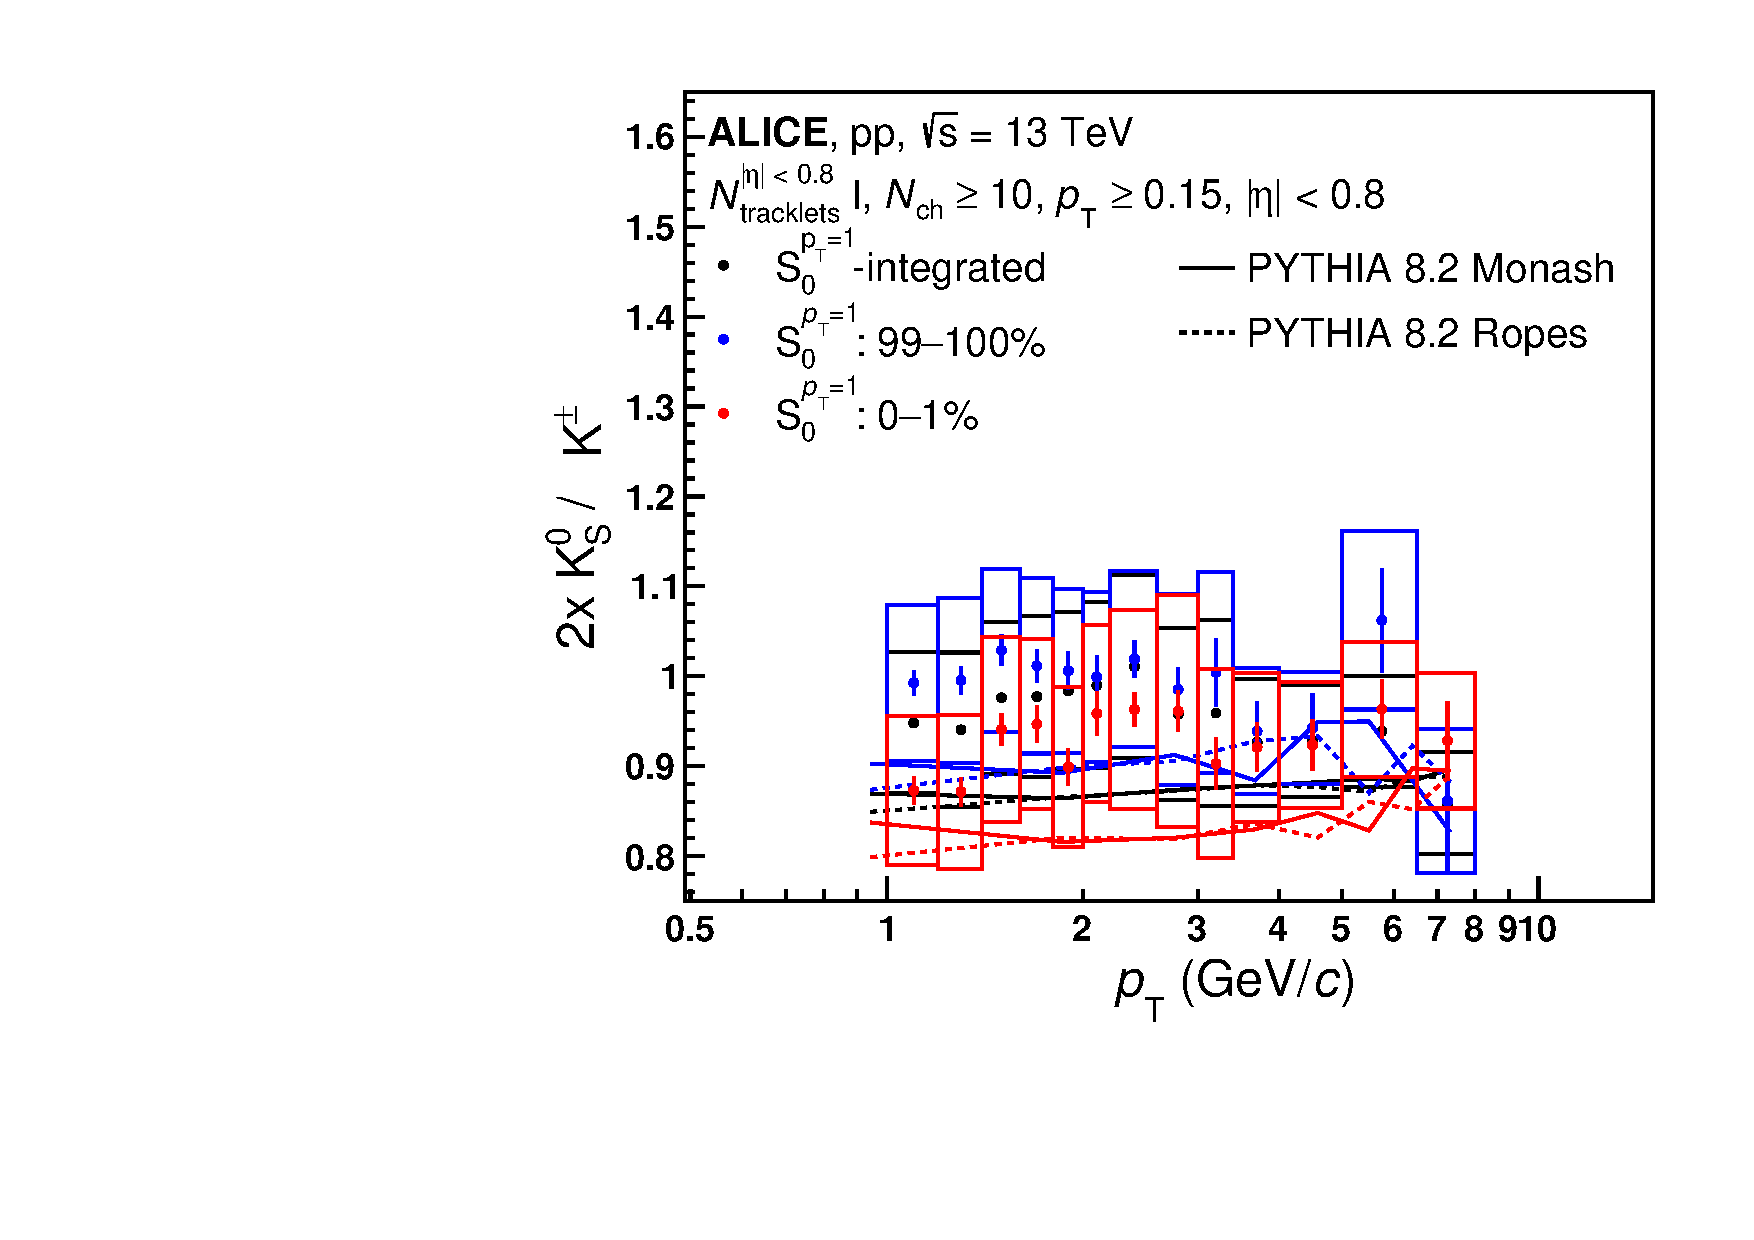
\includegraphics[scale=0.396]{figures/KtoK_NCharged01_spher1.pdf}
    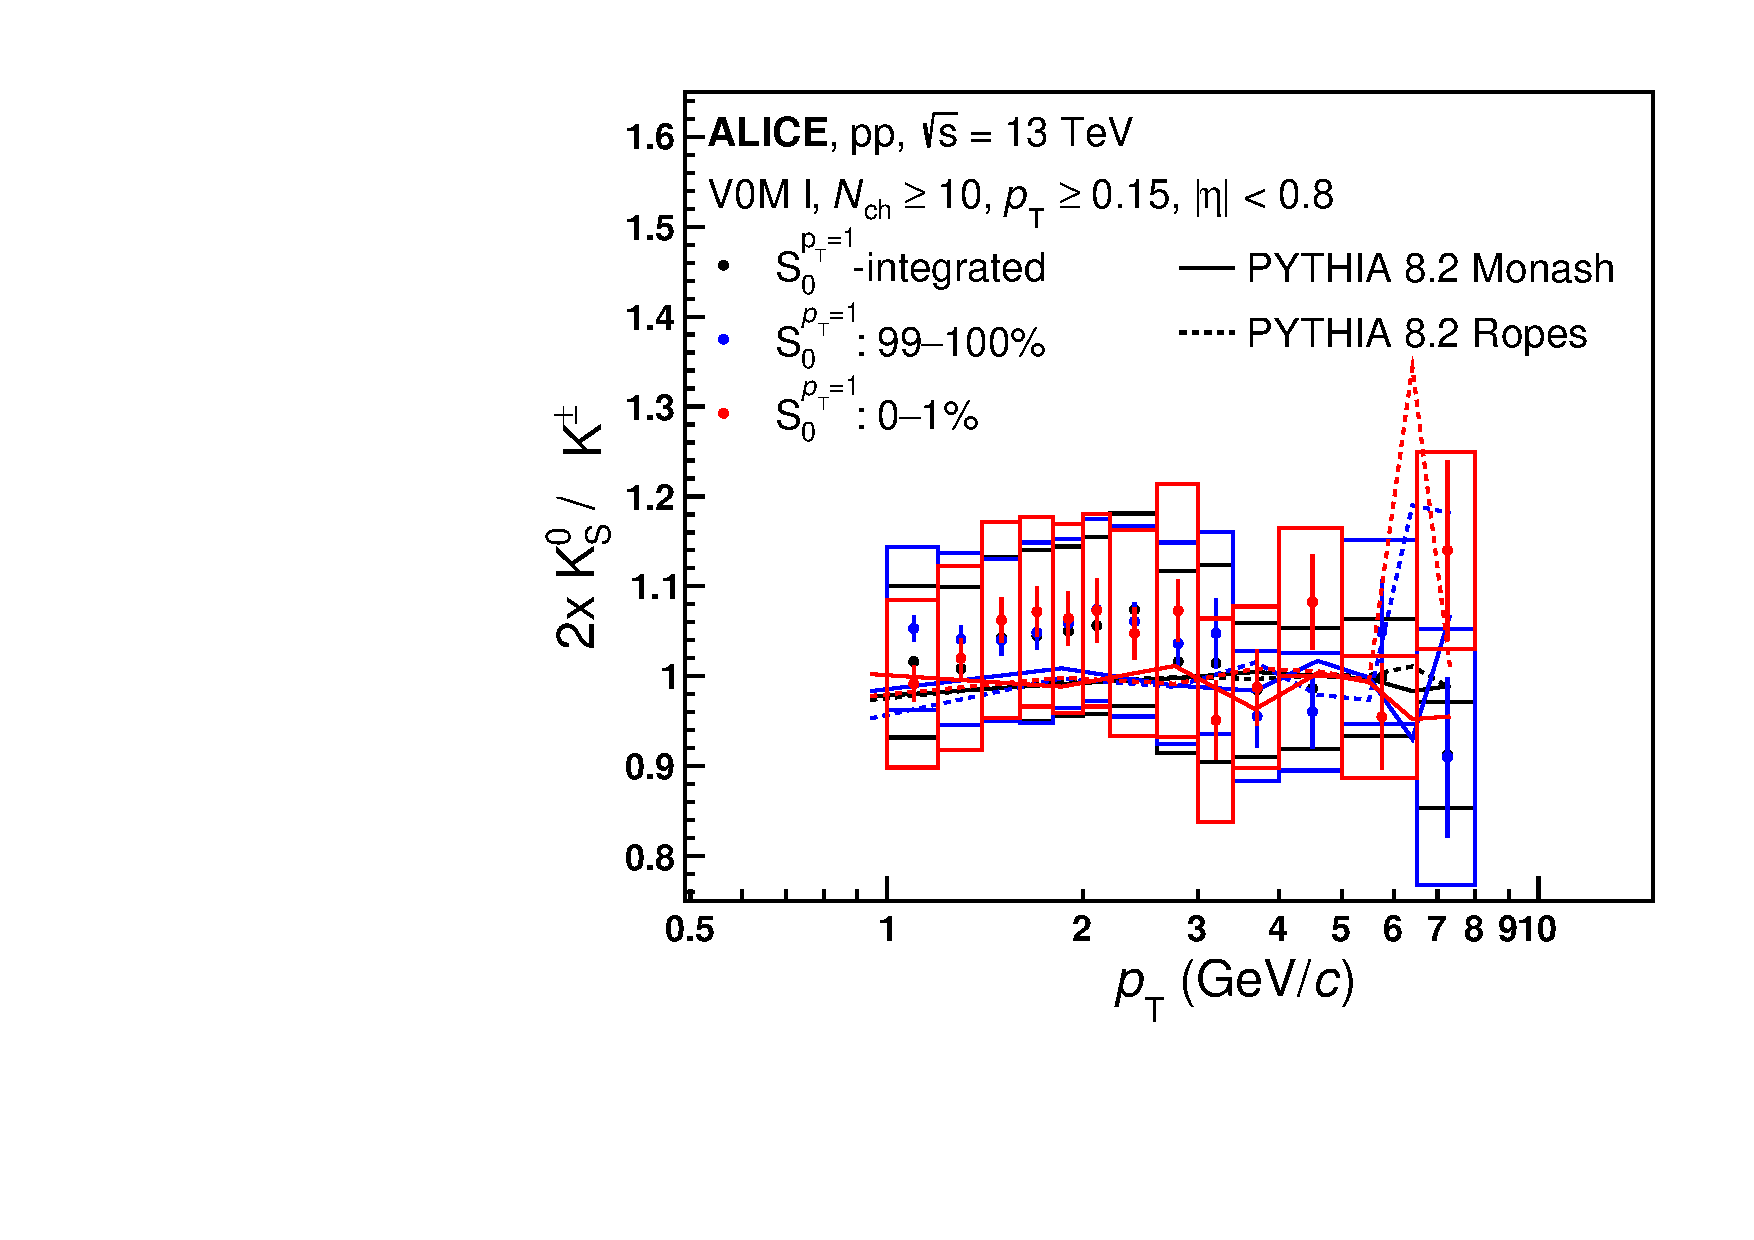
\includegraphics[scale=0.396]{figures/KtoK_V0M01_spher1.pdf}
    \caption{The neutral-to-charged \kzero/K ratios as a function of different multiplicity estimators and \SOPT. Statistical and total systematic uncertainties are shown by bars and boxes, respectively. The curves represent PYTHIA 8.2 model predictions of the same measurement. }
    \label{Fig:KtoK}
\end{figure}
